\documentclass[13pt]{beamer}
\usetheme{Copenhagen}
\usecolortheme{dolphin}
\usepackage{epsfig}
\usepackage{amsmath}
\usepackage{tabu}
\usepackage{amsfonts}
\usepackage{latexsym}
\usepackage[utf8]{inputenc}
\usepackage{listings}    
\usepackage[catalan]{babel}
\usepackage{newunicodechar} 
\usepackage{graphicx}
\usepackage{subcaption}
\usepackage{float}
\usepackage{pgf, tikz}
\usepackage{listings}
\usepackage{eurosym}
\usepackage{array, multirow}
\usepackage{bbding}
\usepackage{graphicx,wrapfig}

\setcounter{tocdepth}{4}
\setcounter{secnumdepth}{4}
\setlength{\tabcolsep}{2pt}


\newunicodechar{Ŀ}{\L.}
\newunicodechar{ŀ}{\l.}

\definecolor{dkgreen}{rgb}{0,0.6,0}
\definecolor{gray}{rgb}{0.5,0.5,0.5}
\definecolor{mauve}{rgb}{0.58,0,0.82}
\definecolor{maroon}{rgb}{0.5,0,0}
\definecolor{darkgreen}{rgb}{0,0.5,0}

\geometry{paperwidth=150mm,paperheight=115mm}
\lstdefinelanguage{XML}
{
  basicstyle=\fontsize{6}{9}\selectfont\ttfamily,
  morestring=[s]{"}{"},
  morecomment=[s]{?}{?},
  morecomment=[s]{!--}{--},
  commentstyle=\color{darkgreen},
  moredelim=[s][\color{black}]{>}{<},
  moredelim=[s][\color{red}]{\ }{=},
  stringstyle=\color{blue},
  identifierstyle=\color{maroon}
}


\usepackage{hyperref}
\hypersetup{
  colorlinks=false, %set true if you want colored links
  linktoc=all,     %set to all if you want both sections and subsections linked
  linkcolor=blue,  %choose some color if you want links to stand out
}

\title[Generació d'horaris d'institut amb operacions lògiques]{GENERACIÓ D'HORARIS D'INSTITUT AMB OPERACIONS LÒGIQUES}
\author[Ismael El Habri]{Ismael El Habri \\ \footnotesize Tutors: Dr. Josep Suy i Dr. Jordi Coll}
\institute{Universitat de Girona}

\date[KPT 2004] % (optional)
{10 de setembre del 2019}

% \AtBeginSection[]
% {
%   \begin{frame}
%     \frametitle{Índex}
%     \tableofcontents[currentsection]
%   \end{frame}
% }
\begin{document}

\frame{\titlepage}
\begin{frame}
  \frametitle{Índex}
  \tableofcontents
\end{frame}

\section{Introducció}
  \begin{frame}
    \frametitle{Introducció}

    Confecció d'horaris, problema recurrent amb el que es troben els instituts $\Rightarrow$ High School TimeTabling problem (HSTT)\\ ~\\

    \begin{figure}
      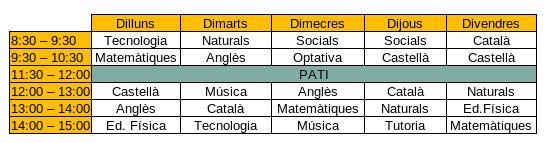
\includegraphics[width=0.6\textwidth]{Diagrames/horari.png}
    \end{figure}
    
    \begin{itemize}
      \item Alta combinatòria i complexitat, és un problema NP-Complet.
      \item Repartir events i recursos de manera viable i tenint en compte preferències del professorat.
      \item Diferents països, diferents necessitats  $\Rightarrow$  més complexitat!
    \end{itemize}
    
    


  \end{frame}
  \subsection{Marc de treball}
  \begin{frame}
    \frametitle{Marc de treball}
    \begin{itemize}
      \item \begin{minipage}{.55\textwidth}
        Grup de recerca de Lògica i Programació
      \end{minipage} 
      \begin{minipage}{.15\textwidth}
        
\includegraphics[width=\textwidth]{Diagrames/LAP.png}
      \end{minipage} 
      \item API SMT desenvolupada pel Dr. Jordi Coll. API per a la codificació de problemes SAT, SMT o MaxSAT, 
      actuant com a interfície per a diferents solvers. En aquest treball s'utilitzarà el Yices 2. 
      També té implementades les diferents implementacions de múltiples restriccions globals.

      \item Com a punt de partida s'ha utilitzat el treball realitzat el 2015 per en Cristòfor Nogueira. 
      Mentre ell ha utilitzat BitVectors i MaxSAT, en aquest treball s'utilitzarà LIA. 
      Així s'han aconseguit uns resultats superiors pel que fa el temps d'execució.
    \end{itemize}

  \end{frame}
  
  \subsection{Objectius}

  \begin{frame}
    \frametitle{Objectius}

\scalebox{1.25}{\begin{minipage}{\textwidth}

    \begin{itemize}
    
      \item Aprofundir sobre el tema.
       \begin{itemize}
        \item Problema de generació d'horaris d'institut.
        \item Problemes de satisfacció de restriccions(CSP).
        \item Tècniques per resoldre problemes CSP com ara SAT i extensions.
       \end{itemize}
      \item Crear un generador.
    
    \end{itemize}
  \end{minipage}}
          
  \end{frame}
  
  \subsection{Metodologia}
  \begin{frame}
    \frametitle{Metodologia}

\scalebox{1.25}{\begin{minipage}{\textwidth}
    \begin{itemize}
      \item Estudi del treball previ i estat de l'art
      \begin{enumerate}
        \item SAT
        \item MaxSAT
        \item SMT
      \end{enumerate}
      \item Entregues periòdiques
      \item Prototipatge
    \end{itemize}
  \end{minipage}}
  \end{frame}

  \subsection{Planificació}
  \begin{frame}
    \frametitle{Planificació}

\scalebox{1.25}{\begin{minipage}{\textwidth}
    \begin{enumerate}
      \item Estudi del problema i la seva duresa.
      \item Disseny i implementació
      \begin{enumerate}
        \item Parser i estructura de dades
        \item Codificació model i restriccions
        \item Tractament de la solució
      \end{enumerate}
      \item Estudi dels resultats
        \end{enumerate}
      \end{minipage}}
  \end{frame}

  \subsection{Pressuposts}
  \begin{frame}{Pressuposts}
    \begin{center}
      \begin{tabular}{|| c | c | c | c||} 
      \hline
       & \euro/h & Hores & Cost \\ [0.5ex] 
      \hline\hline
      Programador & 14 & 260 & 2520 \\ [1ex] 
      \hline
     \end{tabular}
     \end{center}
  
     \begin{center}
      \begin{tabular}{|| c | c |} 
      \hline
       & Cost Total \\ [0.5ex] 
      \hline\hline
      Ordinador Principal & 828  \\ [1ex] 
      Ordinador Portatil Secundari & 200 \\ [1ex] 
      \hline\hline
      Total & 1028 \\
      \hline
     \end{tabular}
     \end{center}
  
     \begin{center}
      \begin{tabular}{|| c | c ||} 
      \hline
       & Hores \\ [0.5ex] 
      \hline\hline
      Josep Suy & 30 \\ [1ex] 
      Jordi Coll & 20 \\ [1ex] 
      \hline
     \end{tabular}
     \end{center}
  \end{frame}

  \section{Implementació}
  \begin{frame}
    \frametitle{Índex}
    \tableofcontents[currentsection]
  \end{frame}
  
  \begin{frame}
  \frametitle{Implementació: Esquema}
    \begin{figure}[p]
      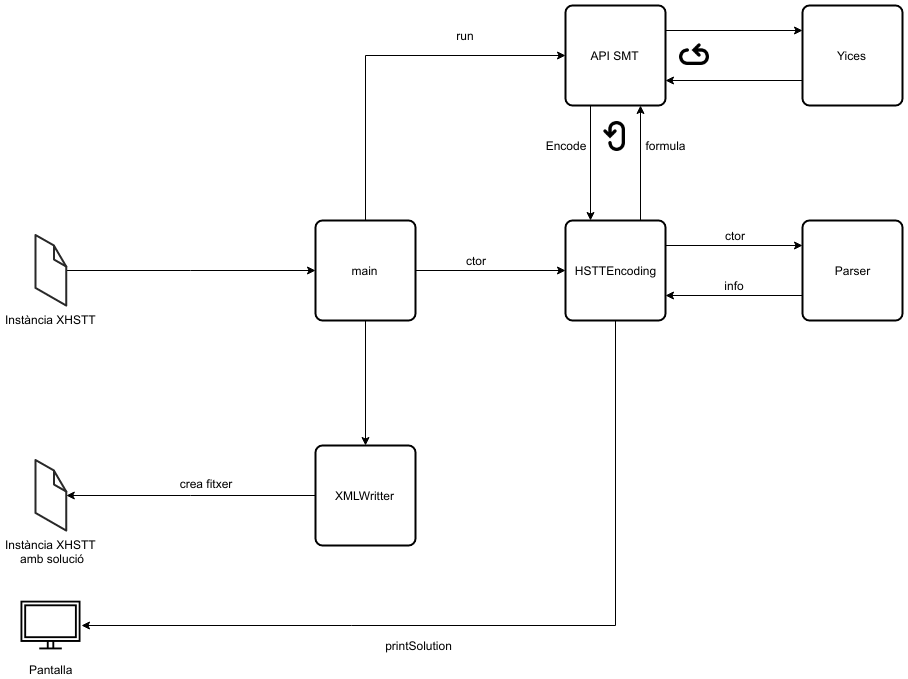
\includegraphics[width=0.85\textwidth]{Diagrames/Arqui2.png}
      \label{fig:procs}
    \end{figure}
  \end{frame}

  \begin{frame}
    \frametitle{Implementació: Model de dades}
    \begin{figure}[p]
      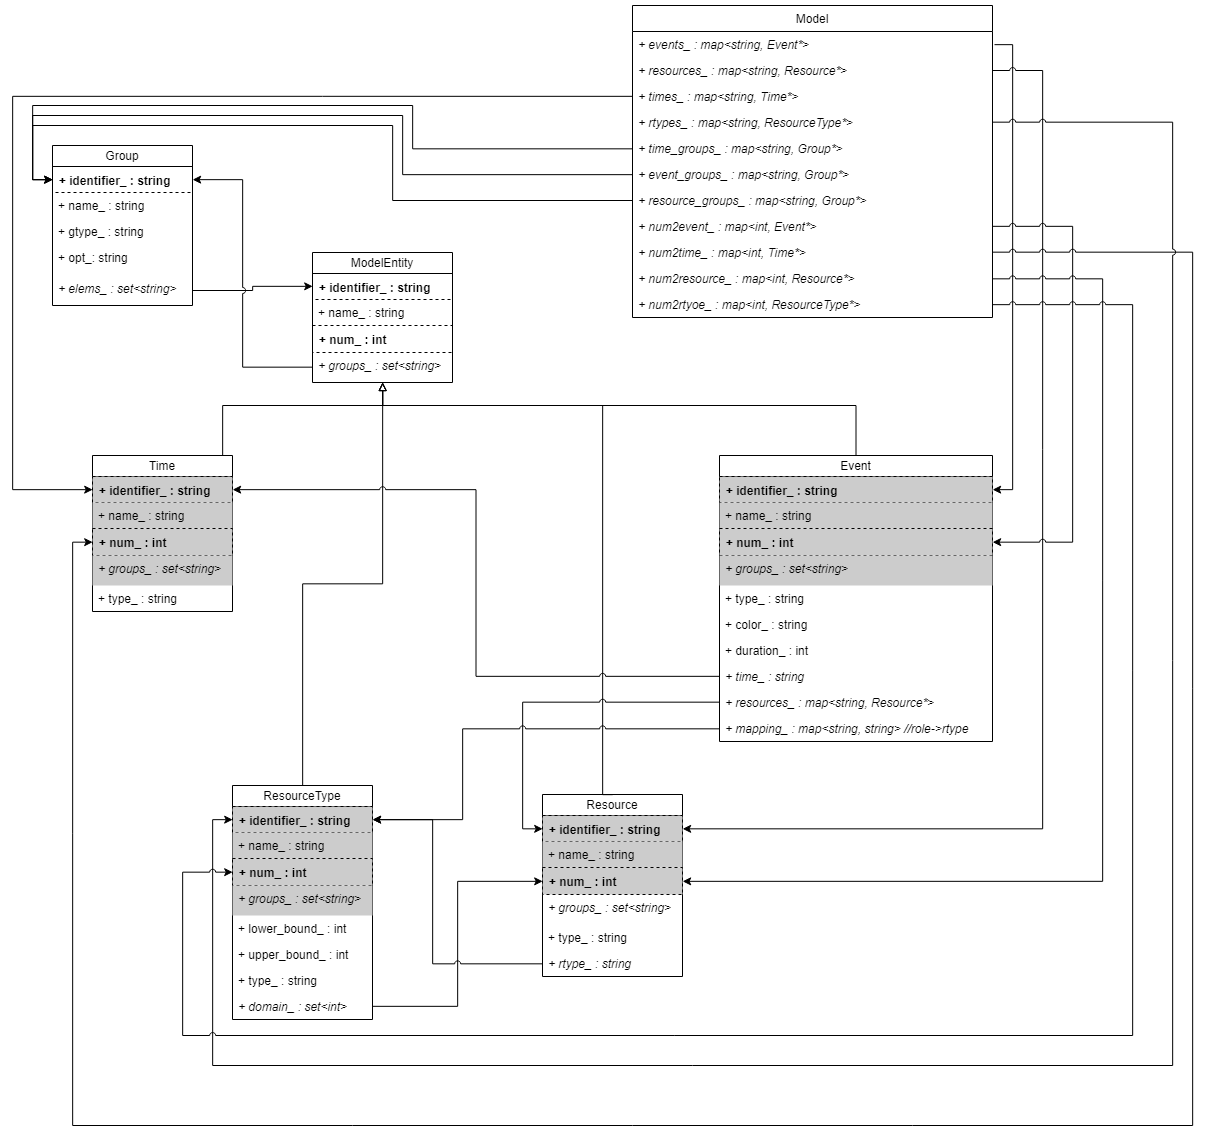
\includegraphics[width=0.75\textwidth]{Diagrames/ModelDades.png}
      \label{fig:procs}
    \end{figure}
  \end{frame}

  \begin{frame}
    \frametitle{Implementació: Model d'objectes}
    \begin{figure}[p]
      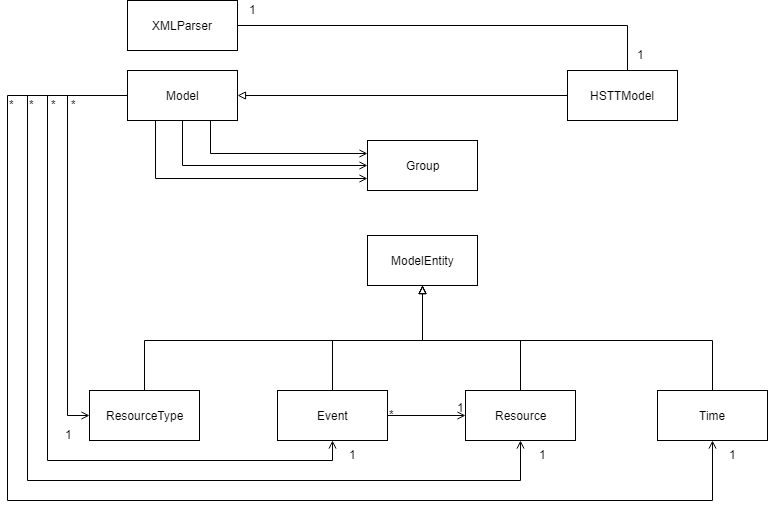
\includegraphics[width=0.85\textwidth]{Diagrames/UMLKai.png}
      \label{fig:procs}
    \end{figure}
  \end{frame}


  
  \subsection{Parser}
  
  \begin{frame}[fragile]
    \frametitle{Parser}
    \begin{minipage}{.5\textwidth}
      \lstinputlisting[language=XML]{listings/resource_ex.xml}      
    \end{minipage}
    \begin{minipage}{.4\textwidth}
      \lstinputlisting[language=XML]{listings/constraint4.xml}      
    \end{minipage}
    ~\\
    Instància XHSTT $\Rightarrow$ dades + restriccions
  \end{frame}

  \subsection{Model}
   
  \begin{frame}
    \frametitle{Model}

    \begin{itemize}
      \item $Xt_{0,0} . . . Xt_{|Events|-1,|Times|-1}$\\Cada variable ens indica si en un espai de temps, es dona lloc l'event corresponent.
      \item $Xs_{0,0} . . . Xs_{|Events|-1,|Times|-1}$\\Cada variable ens indica si en un espai de temps, comença l'event corresponent.
      \item $Xd_{0,1,0} . . . Xd_{|Events|-1, event.duration, |Times|-1}$\\ 
      Cada variable ens indica si comença una lliçó de la durada i en l'espai de temps que representa la variable. 
    \end{itemize}
  \end{frame}

  \begin{frame}
    \frametitle{Clàusules de Channeling} 
    \begin{figure}[p]
      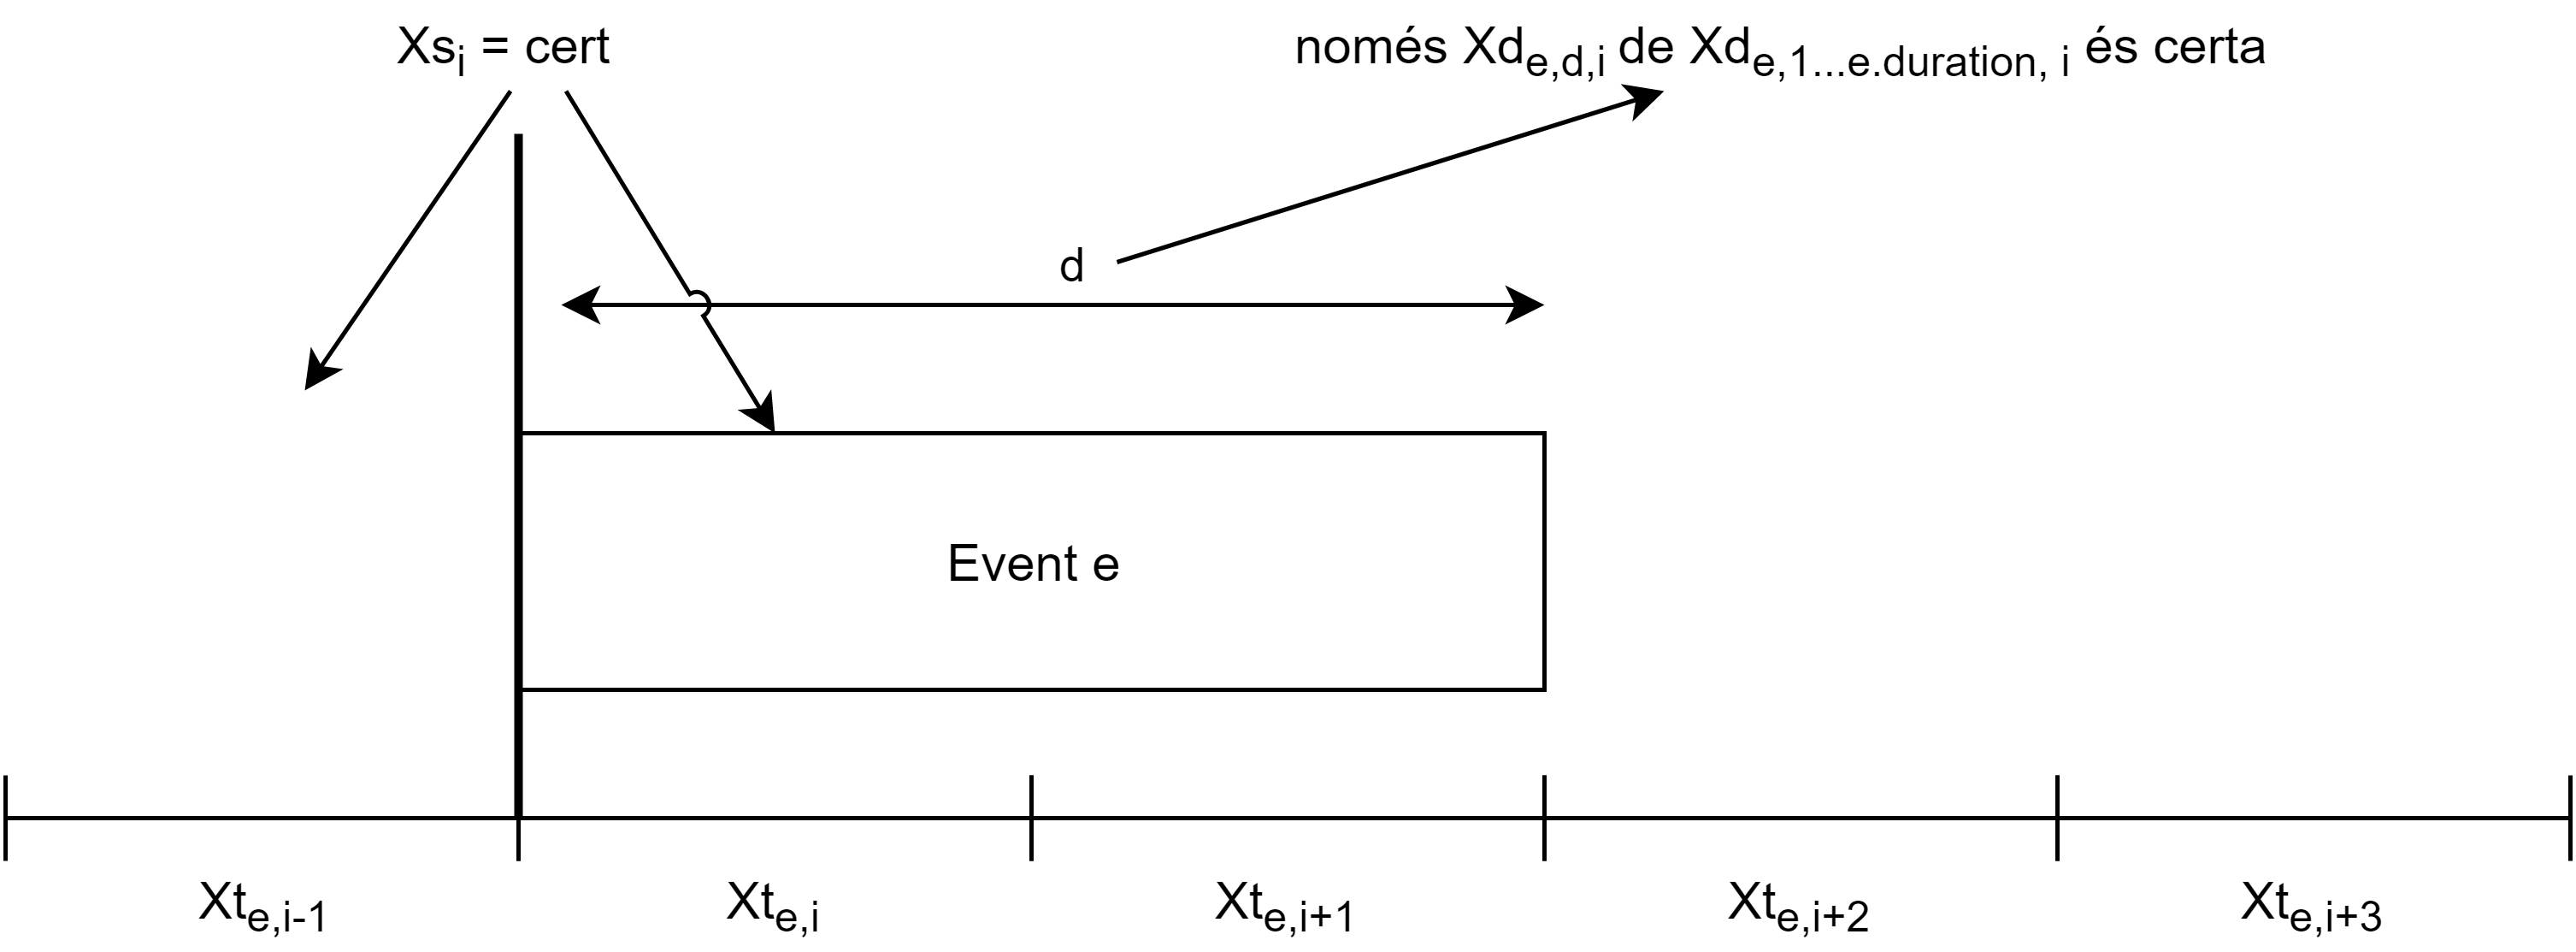
\includegraphics[width=0.85\textwidth]{Diagrames/DiagramaChanneling.png}
      \label{fig:procs}
    \end{figure} 

  
    \end{frame}
  

  \begin{frame}
  \frametitle{Clàusules de Channeling}  

  \begin{itemize}
    \item Si un event comença a una hora determinada, llavors té una duració: 
  \begin{center} 
  $\forall e \in 0 ... |Events|-1$ $\forall i \in 0 ... |Times|-1$ \\
  $Xs_{e,i} \rightarrow exactly\_one(\{Xd_{e,1 ... e.duration,i}\})$\end{center}
    \item Si un event té lloc a t però no a t-1, és que comença: 
  \begin{center} 
  $\forall e \in 0 ... |Events|-1$ $\forall i \in 0 ... |Times|-1$ \\$(Xt_{e,i} \land \neg Xt_{e,i-1}) \rightarrow Xs_{e,i}$ \end{center}
    \item Si un event comença amb duració d, llavors té lloc en d hores consecutives: 
    \begin{center} 
      $\forall e \in 0 ... |Events|-1$ $\forall d \in 1 ... e.duration$ $\forall i \in 0 ... |Times|-1$ $\forall j \in i ... i+d-1$ \\
      $Xd_{e,d,i} \rightarrow Xt_{e,j}$    
    \end{center}
  \end{itemize}

  \end{frame}

  \subsection{Restriccions}

  
  \begin{frame}{Restriccions}{Assign Times Constraint i Distribute Split Constraint}

    \textbf{Assign Times Constraint}\\
    Restricció per imposar que tots els events se'ls assigni els espais de temps corresponents. 
    \[
      \forall e \in Events \ exactly\_k(\{Xt_{e,0 ... |Times|-1}\}, e.duration)
    \]
    \textbf{Distribute Split Constraint}\\
    Restricció que limita el nombre de events d'una duració determinada, per tant limita la cardinalitat de variables $Xd$.

      \begin{align*}
      \forall e \in Events \ at\_most\_k(\{Xd_{e,d,0 ... |Times|-1}\}, max) \quad \quad si \ max<\frac{e.duration}{d}\\
      \forall e \in Events \ at\_most\_k(\{Xd_{e,d,0 ... |Times|-1}\}, min) \quad \quad \quad si \ min>0\\
      \end{align*}

  \end{frame}

  \begin{frame}{Restriccions}{Split Events Constraint}
    Limita la manera en com es fragmenten els events.
    \\\textbf{Nombre de sessions:}
    \begin{gather*}
      \forall e \in Events \ at\_most\_k(\{Xs_{e,0} . . . Xs_{e,|Times|-1}\}, MaximumAmount)\\
      \forall e \in Events \ at\_least\_k(\{Xs_{e,0} . . . Xs_{e,|Times|-1}\}, MinimumAmount)
    \end{gather*}
  
    \textbf{Durada de les sessions:}
    \begin{gather*}
      \forall e \in Events \ \forall d \notin MinimumDuration...MaximumDuration \land d \in 1 ... e.duration  \\
      \forall t \in 0...|Times|-1 \quad (\neg Xd_{e,d,t})
    \end{gather*}  
  \end{frame}

  \begin{frame}{Restriccions}{Prefer Times Constraint i Spread Events Constraint}
    \textbf{Prefer Times Constraint}\\
    Restricció que indica en quins espais de temps no es poden programar certes sessions.
    \begin{gather*}
      \forall e \in Events \ \forall t \in Times \land t \notin Ta \\ (\neg Xd_{e,d,t})
    \end{gather*}
    \textbf{Spread Events Constraint}\\
    Restricció posa límits en el nombre de sessions de 
    cada event que es poden celebrar en certs dies.
        \begin{align*}
          \forall e \in Events \ &\forall g \in Tg \\
          &at\_most\_k(\{Xs_{e,t} | t \leftarrow g\}, max)\\
          \forall e \in Events \ &\forall g \in Tg \\
          &at\_least\_k(\{Xs_{e,t} | t \leftarrow g\}, max)
        \end{align*}    
  \end{frame}

  \begin{frame}{Restriccions}{Avoid Clashes Constraint i Avoid Unavailable Times Constraint}  
      \textbf{Avoid Clashes Constraint}\\
      Aquesta restricció imposa que certs recursos no poden tenir assignats més d'un event al mateix temps. 
        \begin{align*}
          \forall r \in Resources \ & \forall t \in Times \\
          &at\_most\_one(\{Xt_{e,t} | e \leftarrow E_r\})
        \end{align*}
        \textbf{Avoid Unavailable Times Constraint}\\
        Restricció que indica que hi ha certs espais de temps durant les quals no podem utilitzar certs recursos.
        \begin{align*}
          \forall r \in Resources \ \forall t \in T \ \forall e \in E_r \quad
          (\neg Xt_{e,t})
        \end{align*}  
  \end{frame}
  \begin{frame}{Restriccions}{Limit Idle Times Constraint}
    Restricció que limita el nombre d'espais de temps lliure entre dos espais de temps ocupats a l'horari de certs recursos. 
    
    Per a cada recurs $r$ es fan les clàusules següents:

       \begin{align*}
        \forall g \in Tg \ \forall t \in g \ \forall e \in E_r& \\
        &(Idle_i \rightarrow \neg Xt_{e, t}) & si \ \ (B_t \neq \emptyset \ \& A_t \neq \emptyset) \\
        \forall g \in Tg \ \forall t \in g  \ & \\
        & (\neg Idle_t \lor \{Xt_{e\leftarrow E_r,b\leftarrow B_t}\}) & si \ \ (B_t \neq \emptyset)\\
        \forall g \in Tg \ \forall t \in g & \\
        & (\neg Idle_t \lor \{Xt_{e\leftarrow E_r,a\leftarrow A_t}\}) & si \ \ (A_t \neq \emptyset)\\
        \forall g \in Tg \ \forall t \in g \ \forall b \in B_t \ & \forall a \in A_t \\
        \forall e1 \in E_r \ \forall e_2 \in E_r \  &\forall e_3 \in E_r \\
        & (\neg Xt_{e_{1}, t} \land Xt_{e_2, b} \land \neg Xt_{e_3, a} \rightarrow Idle_t) & si \ \ (B_t \neq \emptyset \ \& A_t \neq \emptyset)
       \end{align*}
    
      \end{frame}
      \begin{frame}{Restriccions}{Limit Idle Times Constraint}
       Un cop definides i lligades les variables auxiliars cal imposar les restriccions de cardinalitat:
    
       \begin{align*}
        \forall r \in Resources &\\
        & at\_most\_k(\{ Idle_t | t \leftarrow Times\}, max) \\
        & at\_least\_k(\{ Idle_t | t \leftarrow Times\}, min)
       \end{align*}
  
  \end{frame}
  \begin{frame}
    \frametitle{Restriccions}

    \begin{itemize}
    
      \item Cluster Busy Times Constraint \\
      Restricció que imposa límits sobre el nombre de dies en què un recurs pot estar ocupat.\\
      Per a cada recurs $r$ es fan les clàusules següents:
      
      \begin{align*}
        \forall g \in Tg & \\
        &(\neg Busy_g \lor (\forall e \in E_r \ \forall t \in g \quad Xt_{e,t}))\\
        \forall g \in Tg \ \forall t \in g \ \forall e \in E_r &\\
        & (\neg Xt_{e,t} \lor Bsuy_g)
      \end{align*}
    
      Un cop definides i lligades les variables auxiliars l'únic que queda és, per cada recurs, imposar les restriccions de cardinalitat:
      \begin{align*}
        \forall r \in Resources &\\
        & at\_most\_k(\{ Busy_g | g \leftarrow Tg\}, max) \\
        & at\_least\_k(\{ Busy_g | g \leftarrow Tg\}, min)
       \end{align*}
          
    \end{itemize}
  
  \end{frame}

  \begin{frame}{Funció objectiu}
    Per cada clàusula \textit{soft} afegim una variable auxiliar $aux_i$ i ens guardem el pes $w_i$ d'aquesta.
    \\ Per a la optimització afegim la següent clàusula pseudobooleana, per a $n$ clàusules 
    \textit{soft}:\\ \[
        aux_{0}w_{0} + . . .  + aux_{n-1}w_{n-1} \leq UPPERBOUND
    \]
  
  \end{frame}


  \section{Conclusions i Resultats}
  \begin{frame}
    \frametitle{Índex}
    \tableofcontents[currentsection]
  \end{frame}
  \subsection{Resultats}

  \begin{frame}{Resultats}{Diferents Encodings}
    \begin{itemize}
      \item $at\_most\_one$
      \begin{itemize}
        \item Quadràtic
        \item Logarítimic
        \item Ladder
        \item Heule
      \end{itemize}
      \item Restriccions de cardinalitat
      \begin{itemize}
        \item Sorter
        \item Totalizer
      \end{itemize}
    \end{itemize}
  \end{frame}
  
  \begin{frame}{Resultats}{Temps de resolució}
    \centering    
      \begin{tabular} { c | c c | c c | c c}
        \multirow{2}{*}{Encodings} & 
        \multicolumn{2}{c | }{BrazilInstance1} & \multicolumn{2}{c | }{BrazilInstance2} & \multicolumn{2}{c}{BrazilInstance3} \\ \cline{2-7}
        &\textit{Sorter} & \textit{Totalizer} & \textit{Sorter} & \textit{Totalizer} & \textit{Sorter} & \textit{Totalizer} \\
        \hline
        Quadràtic &  \textbf{1.052} & 1.126 & 6.450 &6.136 &10.331& \textbf{9.743}   \\
        Logarítmic & 1.126 & 1.184 & 6.151 &\textbf{6.080} &10.989& 10.784 \\
        Ladder &     1.275 & 1.300 & 6.084 &6.123 &12.492& 15.015  \\
        Heule &      1.242 & 1.105 & 6.437 &7.142 &11.815& 10.604 \\
      \end{tabular}
     ~\\~\\~\\
      \begin{tabular} { c | c c | c c | c c | c c}
        \hline
        \multirow{2}{*}{Encodings} & 
        \multicolumn{2}{c | }{BrazilInstance4} & \multicolumn{2}{c | }{BrazilInstance5} & \multicolumn{2}{c | }{BrazilInstance6} & \multicolumn{2}{c}{BrazilInstance7}\\ \cline{2-9}
        &\textit{Sorter} & \textit{Totalizer} & \textit{Sorter} & \textit{Totalizer} & \textit{Sorter} & \textit{Totalizer} & \textit{Sorter} & \textit{Totalizer} \\
        \hline
        Quadràtic &   \textbf{02:56.91} & 05:19.96 & 28.63 & \textbf{28.235}&  \textbf{35.45}  &36.191  &  01:52.45 & 01:50.34 \\
        Logarítmic &  11:38.62 & 24:33.60 & 28.753& 28.768 & 39.163 &36.309  &  \textbf{01:48.02} & 01:48.46\\
        Ladder &      Timeout &  07:24.02 & 31.018& 31.006 & 39.797 &01:06.33&  02:22.87 & 02:27.35 \\
        Heule &       05:03.38 & 25:24.81 & 28.934& 29.046 & 40.441 &36.852  &  02:38.68 & 02:38.79\\
      \end{tabular}
  \end{frame}
  
  
  \begin{frame}{Resultats}{Variables generades}
    \centering
      \begin{tabular} { c | c c | c c | c c}
        \multirow{2}{*}{Encodings} & 
        \multicolumn{2}{c | }{BrazilInstance1} & \multicolumn{2}{c | }{BrazilInstance2} & \multicolumn{2}{c}{BrazilInstance3} \\ \cline{2-7}
        &\textit{Sorter} & \textit{Totalizer} & \textit{Sorter} & \textit{Totalizer} & \textit{Sorter} & \textit{Totalizer} \\
        \hline
        Quadràtic &  131,391 & \textbf{131,349} & \textbf{924,783} & 924,807 & 1,223,115 & \textbf{1,223,085} \\
        Logarítmic & 131,941 & 131,899 & 926,208 & 926,232 & 1,224,765 & 1,224,735\\
        Ladder &     132,166 & 132,124 & 927,433 & 927,457 & 1,225,965 & 1,225,935 \\
        Heule &      131,841 & 131,799 & 927,283 & 927,307 & 1,225,615 & 1,225,585\\
      \end{tabular}
  \end{frame}

  \begin{frame}{Resultats}{Variables generades}
      \centering
      \begin{tabular} { c|c c|c c}
        \multirow{2}{*}{Encodings} & 
        \multicolumn{2}{c | }{BrazilInstance4} & \multicolumn{2}{c }{BrazilInstance5} \\ \cline{2-5}
        &\textit{Sorter} & \textit{Totalizer} & \textit{Sorter} & \textit{Totalizer}    \\ 
        \hline
        Quadràtic &  \textbf{3,710,406} & 3,710,472  & \textbf{3,535,238} & \textbf{3,535,238}     \\ 
        Logarítmic & 3,713,081 & 3,713,147  & 3,537,838 & 3,537,838     \\ 
        Ladder &     Timeout	  & 3,715,947 & 3,540,088 & 3,540,088     \\ 
        Heule &      3,715,756 & 3,715,822  & 3,539,588 & 3,539,588     \\ 
      \end{tabular}

      ~\\~\\~\\

     \begin{tabular}  { c|c c|c c}
       \multirow{2}{*}{Encodings} 
                          & \multicolumn{2}{c | }{BrazilInstance6} & \multicolumn{2}{c}{BrazilInstance7}\\ \cline{2-5}
                          & \textit{Sorter} & \textit{Totalizer} & \textit{Sorter} & \textit{Totalizer} \\
       \hline
       Quadràtic          & \textbf{4,652,421}	& 4,652,523 & \textbf{9,835,793} & \textbf{9,835,793} \\
       Logarítmic         & 4,655,646	& 4,655,748 & 9,840,268 & 9,840,268 \\
       Ladder             & 4,658,321	& 4,658,423 & 9,844,718 & 9,844,718 \\
       Heule              & 4,657,946	& 4,658,048 & 9,844,718 & 9,844,718 \\
     \end{tabular}
    
  \end{frame}


  \begin{frame}{Resultats}{Clàusules generades}
    \centering
    \begin{tabular} { c | c c | c c | c c}
      \multirow{2}{*}{Encodings} & 
      \multicolumn{2}{c | }{BrazilInstance1} & \multicolumn{2}{c | }{BrazilInstance2} & \multicolumn{2}{c}{BrazilInstance3} \\ \cline{2-7}
      &\textit{Sorter} & \textit{Totalizer} & \textit{Sorter} & \textit{Totalizer} & \textit{Sorter} & \textit{Totalizer} \\
      \hline
      Quadràtic &  703,680 & 703,666 & 3,556,395 &	3,556,497 & 5,960,643 & 5,960,705 \\
      Logarítmic & 704,130 & 704,116 & 3,556,120 &	3,556,222 & 5,961,218 & 5,961,280 \\
      Ladder &     703,705 & 703,691 & 3,553,195 &	3,553,297 & 5,958,443 & 5,958,505 \\
      Heule &      703,380 & \textbf{703,366} & \textbf{3,553,045} &	3,553,147 & \textbf{5,958,093} & 5,958,155 \\
    \end{tabular}
  \end{frame}

  \begin{frame}{Resultats}{Clàusules generades}
    \centering
    \begin{tabular} { c|c c|c c}
      \multirow{2}{*}{Encodings} & 
      \multicolumn{2}{c | }{BrazilInstance4} & \multicolumn{2}{c }{BrazilInstance5} \\ \cline{2-5}
      &\textit{Sorter} & \textit{Totalizer} & \textit{Sorter} & \textit{Totalizer}    \\ 
      \hline
      Quadràtic &  14,414,235 & 14,414,410 & 16,200,714 & 16,200,714     \\ 
      Logarítmic & 14,412,135 & 14,412,310 & 16,200,039 & 16,200,039     \\ 
      Ladder &     Timeout    & 14,405,635 & 16,194,739 & 16,194,739     \\ 
      Heule &      \textbf{14,405,335} & 14,405,510 & \textbf{16,194,239} & \textbf{16,194,239}     \\ 
    \end{tabular}
    ~\\~\\~\\
   \begin{tabular}  { c|c c|c c}
     \multirow{2}{*}{Encodings} 
                        & \multicolumn{2}{c | }{BrazilInstance6} & \multicolumn{2}{c}{BrazilInstance7}\\ \cline{2-5}
                        & \textit{Sorter} & \textit{Totalizer} & \textit{Sorter} & \textit{Totalizer} \\
     \hline
     Quadràtic          & 18,665,275 & 18,665,548 & 38,762,136 & 38,762,136 \\
     Logarítmic         & 18,665,275 & 18,665,548 & 38,760,036 & 38,760,036 \\
     Ladder             & 18,657,900 & 18,658,173 & 38,749,361 & 38,749,361 \\
     Heule              & \textbf{18,657,525} & 18,657,798 & \textbf{38,749,361} & \textbf{38,749,361} \\
   \end{tabular}
 \end{frame}

  \begin{frame}
    \frametitle{Resultats optimització}

    \begin{tabular}  { c| c | c | c}
      Optimitzador & Temps & Cost & Cost de la millor solució\\
      \hline
      BrazilInstance1 & 1:07.66 & 79 & 41\\
      BrazilInstance2 & Timeout & -- & --\\
      BrazilInstance3 & Timeout & -- & --\\
    \end{tabular}
  \end{frame}

  \subsection{Conclusions}

  
  \begin{frame}{Conclusions}
    \begin{itemize}
      \item Estudi, repàs i aplicació de diferents tècniques de programació amb restriccions.
      \item Objectius:
      \begin{itemize}
        \item Resolució en temps raonable $\Rightarrow$ aconseguit
        \item Optimització en temps raonable  $\Rightarrow$ no aconseguit
      \end{itemize}
    \end{itemize}
    \textbf{Treball futur:}\\
    \begin{itemize}
      \item Afegir tipus de instàncies suportades
      \item Intentar provar altres teories de SMT.
      \item Millorar codificacions i model en sí.
      \item Intentar millorar la optimització.
    \end{itemize}


  \end{frame}


  \section{Demostració}
  \begin{frame}
    \frametitle{Demostració}
  \end{frame}




  
\end{document}